\section{Sensors}
\label{sec:Sensors}

\subsection{Potentiometer}
The potentiometer is placed at the corner of the frame which is fixed to an axis and it can be used to measure the actual position of the frame.\\
However its use is restricted to the one-dimensional Cubli, as it is attached and gives only an angle in relation to the base, which is not present in the 3D case.\\
In the project the potentiometer is used to test the dynamics of the Cubli and for feedback in the initial controller design.\\
Since the tests and feedback dependent on the reliability of the potentiometer, a test is carried out to find the voltage to angle conversion along with potential offset, see \appref{potentiometerRes}.

\begin{minipage}{\linewidth}
  	\begin{minipage}{0.45\linewidth}
  		\begin{figure}[H]
  			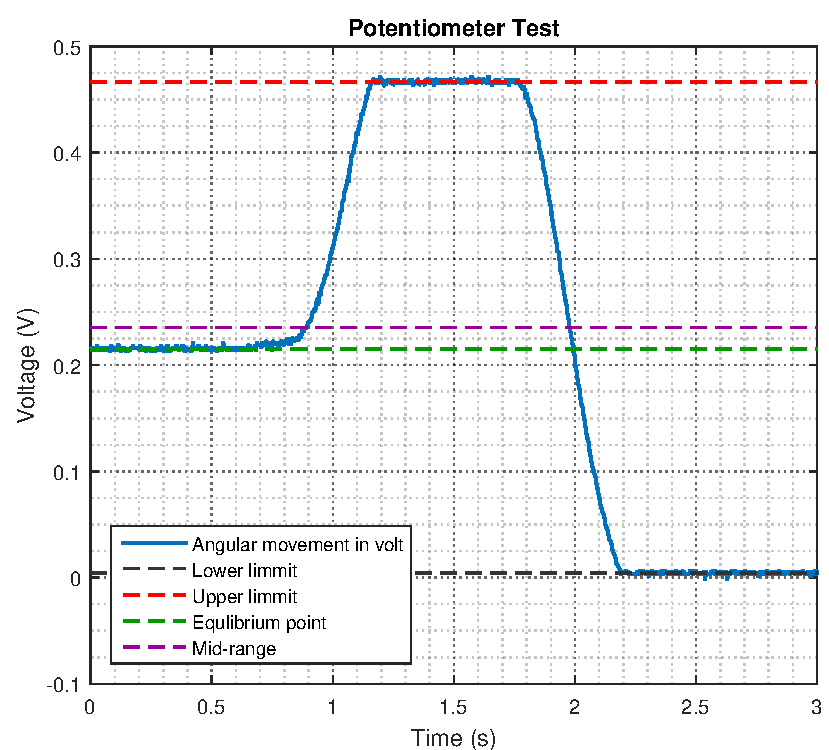
\includegraphics[scale=.5]{figures/PotentiometerResolution}
  			\centering
  			\captionsetup{justification=centering}
  			\captionof{figure}{\\Potentiometer measurements in volts}
  			\label{PotentiometerResolution}
  		\end{figure}\vspace{-5mm}
  	\end{minipage}
  	\hspace{0.03\linewidth}
  	\begin{minipage}{0.45\linewidth}
  		\begin{figure}[H]
  		\vspace{.5cm}
  			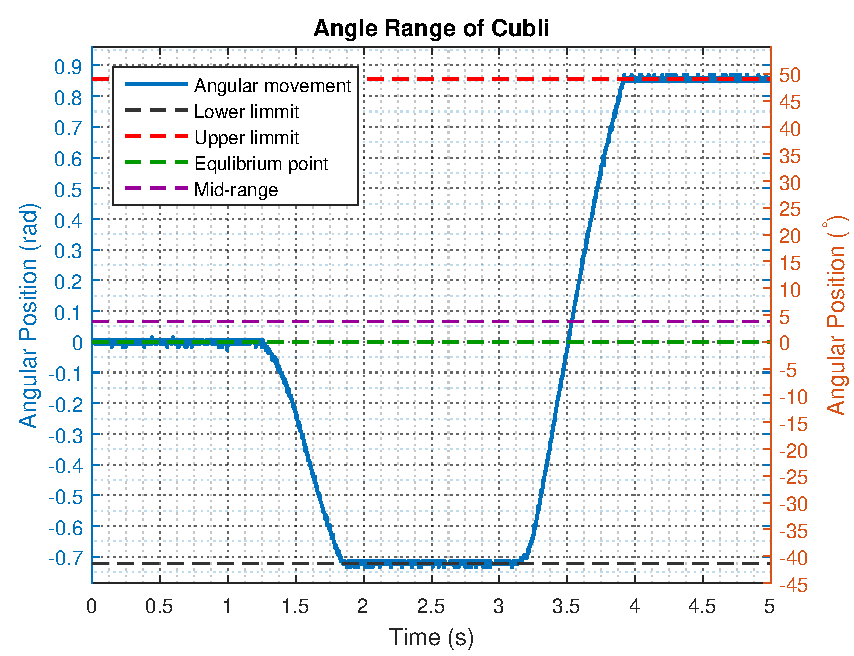
\includegraphics[scale=.5]{figures/PotentiometerResolutionDegRad}
  			\centering
  			\captionsetup{justification=centering}
  			\vspace{-.5cm}
  			\captionof{figure}{\\Potentiometer measurements converted to radians and degrees}
  			\label{PotentiometerResolutionRadDeg}
  		\end{figure}\vspace{-5mm}
  	\end{minipage}
\end{minipage}

The results of this test is shown above in \figref{PotentiometerResolution}, where the reference lines reveals an offset between the middle of the range and the equilibrium point of the Cubli frame.\\
This offset, also seen angle offset on \figref{PotentiometerResolutionRadDeg}, exists in the physical position of the frame. When the frame is standing it its equilibrium position it is displaces by approximately \si{3,9} degrees due to uneven distribution of mass around its center.\\
This results in a \si{48,9} degree range to one side of the optimal position and \si{41,1} degrees on the other.\\
To avoid complications it is chosen that the angle-offset must be accounted for such that the equilibrium position of the frame is at angle 0.

\subsection{IMU}
